% ------------------------------------------------------------------------------
% TYPO3 CMS 8 LTS - What's New - Chapter "Backend User Interface" (Dutch Version)
%
% @author	Michael Schams <schams.net>
% @license	Creative Commons BY-NC-SA 3.0
% @link		http://typo3.org/download/release-notes/whats-new/
% @language	English
% ------------------------------------------------------------------------------
% LTXE-CHAPTER-UID:		07b25346-95b1df21-a6ebe09a-49f53f41
% LTXE-CHAPTER-NAME:	Backend User Interface
% ------------------------------------------------------------------------------

\section{Gebruikersinterface backend}
\begin{frame}[fragile]
	\frametitle{Gebruikersinterface backend}

	\begin{center}\huge{\color{typo3darkgrey}\textbf{Gebruikersinterface backend}}\end{center}
	\begin{center}\large{\textit{Het uiterlijk van de TYPO3 CMS backend is weer verbeterd}}\end{center}

\end{frame}

% ------------------------------------------------------------------------------
% LTXE-SLIDE-START
% LTXE-SLIDE-UID:		fc131f99-050d82fd-5776a2f4-c81b0a54
% LTXE-SLIDE-ORIGIN:	fd6d762a-b268caf0-cb6f9195-f553e035 English
% LTXE-SLIDE-TITLE:		Set the alternative backend logo via Extension Manager
% ------------------------------------------------------------------------------
\begin{frame}[fragile]
	\frametitle{Gebruikersinterface backend}
	\framesubtitle{Alternatief logo}

	Het logo linksboven in de backend kan nu in de configuratie van EXT:backend in de extensiemanager
	ingesteld worden.\newline
	Configuratieopties zijn:

	\begin{itemize}
		\item bestand relatief t.o.v. de TYPO3 installatie\newline
			\smaller
				bijv. "\texttt{fileadmin/images/my-background.jpg}"
			\normalsize

		\item pad naar een extensie\newline
			\smaller
				bijv. "\texttt{EXT:my\_theme/Resources/Public/Images/my-background.jpg}"
			\normalsize

		\item een externe bron\newline
			\smaller
				bijv. "\texttt{//example.com/my-background.png}"
			\normalsize

	\end{itemize}

	\begin{figure}
		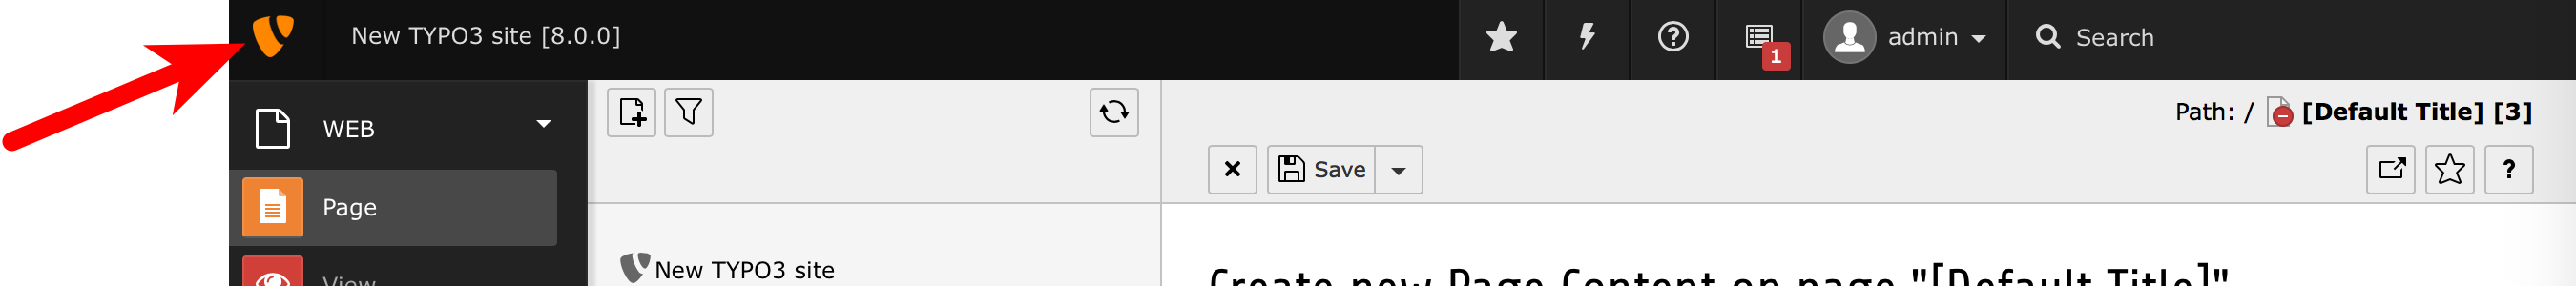
\includegraphics[width=0.7\linewidth]{BackendUserInterface/74109.png}
	\end{figure}

\end{frame}

% ------------------------------------------------------------------------------
% LTXE-SLIDE-START
% LTXE-SLIDE-UID:		fc96e25e-aed70af7-1ca88b77-ce494abb
% LTXE-SLIDE-ORIGIN:	75977160-b74e3317-0f697728-71b501d1 English
% LTXE-SLIDE-TITLE:		Mobile Responsive TYPO3 Backend
% ------------------------------------------------------------------------------

\begin{frame}[fragile]
	\frametitle{Gebruikersinterface backend}
	\framesubtitle{Responsive TYPO3 backend voor mobiel}

	De TYPO3 Backend is nu volledig responsive voor mobiel.

	\begin{figure}
		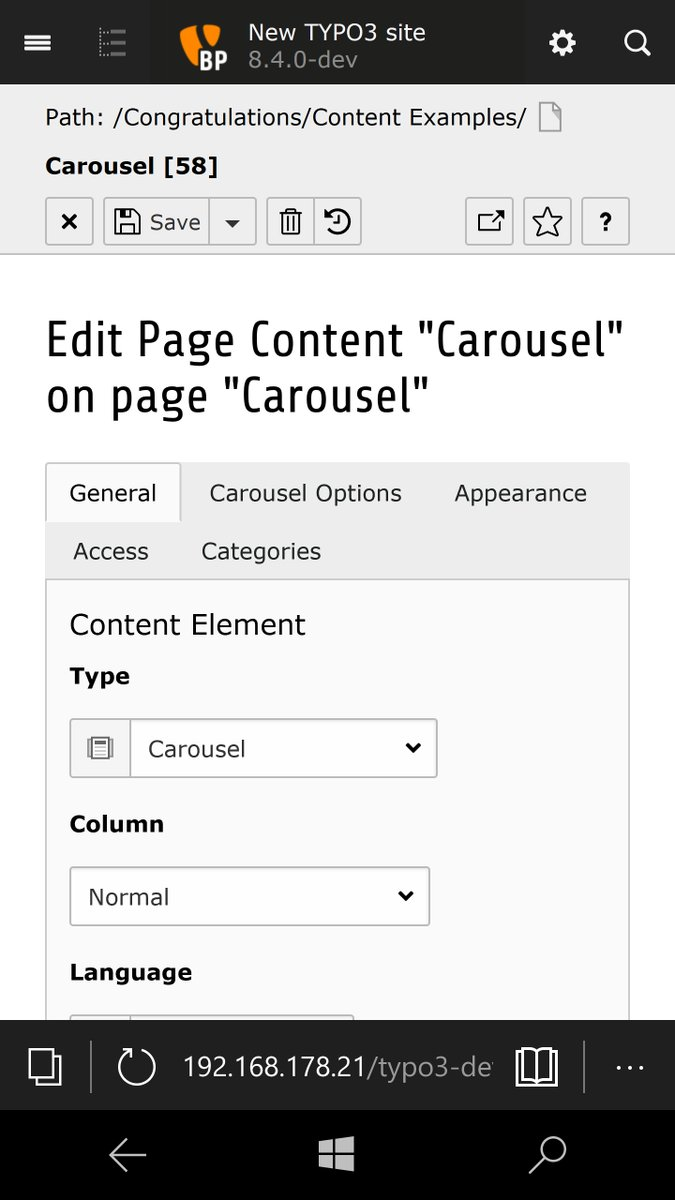
\includegraphics[width=0.25\linewidth]{BackendUserInterface/mobile-responsive-backend.jpg}
	\end{figure}

\end{frame}

% ------------------------------------------------------------------------------
% LTXE-SLIDE-START
% LTXE-SLIDE-UID:		765e01ea-1f4483fb-3f406934-5c367eb6
% LTXE-SLIDE-ORIGIN:	ab5ef36b-c670fbea-fd6d762a-cb6f9195 English
% LTXE-SLIDE-TITLE:		Page module: drag and drop can copy elements
% ------------------------------------------------------------------------------
\begin{frame}[fragile]
	\frametitle{Gebruikersinterface backend}
	\framesubtitle{Elementen kopiëren door verslepen}

	Naast het normale gedrag in de paginamodule dat inhoudselementen \textit{verplaatst} worden door te verslepen
	kunnen nu ook kopieën gemaakt worden: druk de CTRL-toets in tijdens het verslepen om een kopie te maken.
	Na het loslaten wordt de pagina herladen om ervoor te zorgen dat het nieuwe element wordt aangemaakt met alle
	nodige informatie.

	\begin{figure}
		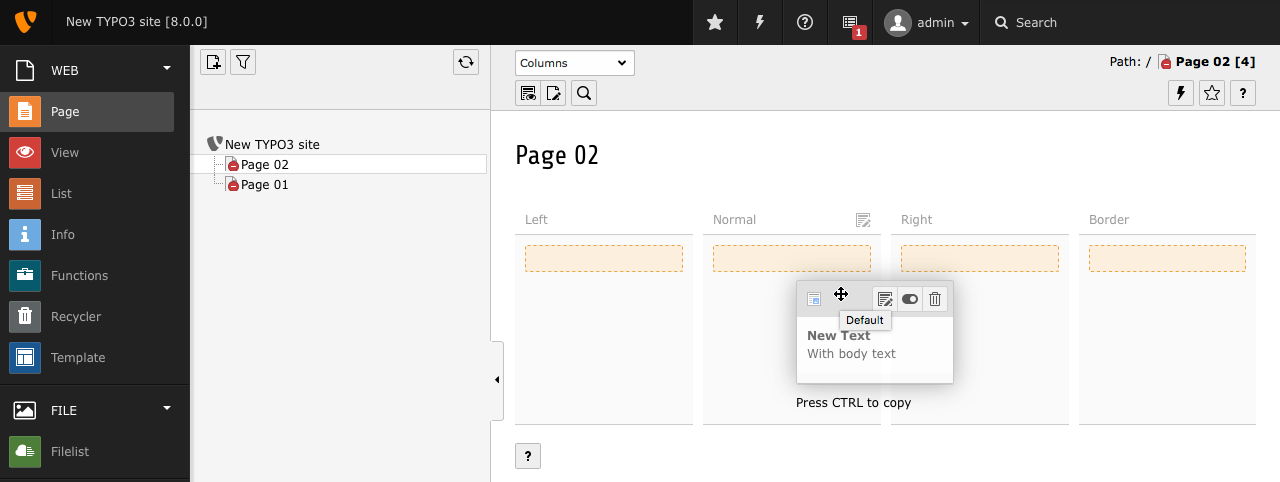
\includegraphics[width=0.7\linewidth]{BackendUserInterface/74179.png}
	\end{figure}

\end{frame}

% ------------------------------------------------------------------------------
% LTXE-SLIDE-START
% LTXE-SLIDE-UID:		32e426f5-f70c933e-f4686ded-9684f87f
% LTXE-SLIDE-ORIGIN:	14d6e262e72f00405d2bedf0096fe043 English
% LTXE-SLIDE-TITLE:		Feature #75880: Image Manipulation - Multiple Cropping Variants (1)
% ------------------------------------------------------------------------------
\begin{frame}[fragile]
	\frametitle{Gebruikersinterface backend}
	\framesubtitle{Beeldbewerking (1)}

	\begin{itemize}

		\item Meerdere verhoudingen kunnen ingesteld worden\newline
			\small(standaard: 16:9, 3:2, 4:3 en 1:1)\normalsize

		\item Redacteuren kunnen een focuspunt instellen (responsive afbeeldingen)\newline
			\small
				(dit deel blijft zichtbaar, ook al is de afbeelding afgesneden,
				bijv. op kleine schermen zoals bij telefoons)
			\normalsize

		\item Ontwikkelaars kunnen \textit{crop-varianten} instellen (bijv. "mobiel",
		 	"PC", etc.) en deze gebruiken in TCA en Fluid-sjablonen

			\begin{lstlisting}
				<f:image image="{data.image}" cropVariant="mobiel" width="800">
				</f:image>
			\end{lstlisting}

			Zie \href{https://docs.typo3.org/typo3cms/extensions/core/8-dev/Changelog/8.6/Feature-75880-ImplementMultipleCroppingVariantsInImageManipulationTool.html}{docs.typo3.org}
			voor meer details.

	\end{itemize}

\end{frame}

% ------------------------------------------------------------------------------
% LTXE-SLIDE-START
% LTXE-SLIDE-UID:		53693f7e-f87a6ab4-66f40eb2-e556c86d
% LTXE-SLIDE-ORIGIN:	23a4baef-462e7d0c-c8cd4cfc-9dac1f99 English
% LTXE-SLIDE-TITLE:		Feature #75880: Image Manipulation - Multiple Cropping Variants (2)
% ------------------------------------------------------------------------------
\begin{frame}[fragile]
	\frametitle{Gebruikersinterface backend}
	\framesubtitle{Beeldbewerking (2)}

	\begin{figure}\vspace*{-0.6cm}
		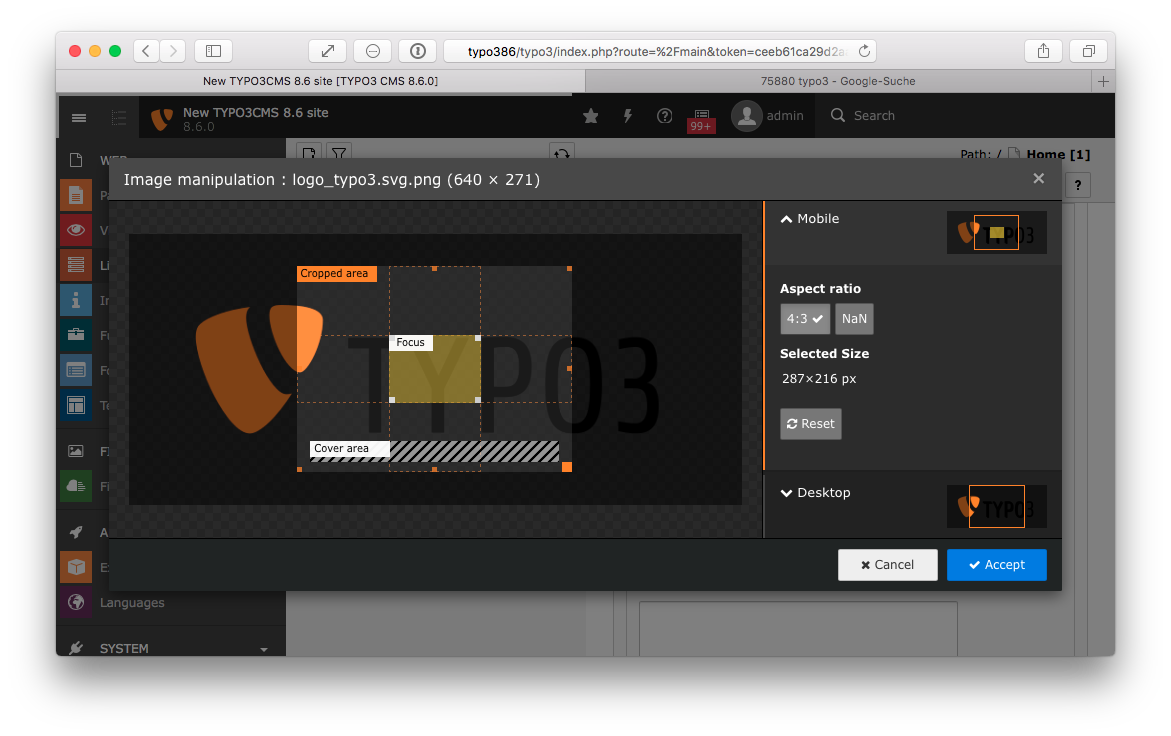
\includegraphics[width=0.90\linewidth]{BackendUserInterface/75880.png}
	\end{figure}

\end{frame}


% ------------------------------------------------------------------------------
% LTXE-SLIDE-START
% LTXE-SLIDE-UID:		f599bd23-2bd7ef5e-fe44bc2a-7dd5c746
% LTXE-SLIDE-ORIGIN:	7cab4dc0-cdfe9472-a3f0a874-dddf137d English
% LTXE-SLIDE-TITLE:		Feature #75581: Cache clearing
% ------------------------------------------------------------------------------
\begin{frame}[fragile]
	\frametitle{Gebruikersinterface backend}
	\framesubtitle{Versimpeld caches legen}

	Het systeem voor het legen van caches is versimpeld door het verwijderen van opties in het
	menu om caches te legen en in de Install Tool.

	\begin{itemize}

		\item \textbf{Frontend caches legen:}\newline
			\small
				Leegt frontend en paginagerelateerde caches, zoals altijd.
			\normalsize

		\item \textbf{Alles caches legen:}\newline
			\small
				Leegt alle systeemgerelateerde caches, inclusief de klasselader, vertalingen,
				extensiesconfiguratiebestandscaches en opcode caches. Het herbouwen van deze caches
				kan even duren.
			\normalsize

	\end{itemize}

	\begin{figure}
		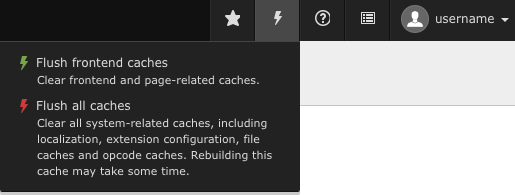
\includegraphics[width=0.45\linewidth]{BackendUserInterface/75581.png}
	\end{figure}

\end{frame}

% ------------------------------------------------------------------------------
% LTXE-SLIDE-START
% LTXE-SLIDE-UID:		3e526159-63e2ed60-0e27ee6b-a174aef4
% LTXE-SLIDE-ORIGIN:	a5b4032f-741b8eea-643674fb-4dc14f50 English
% LTXE-SLIDE-TITLE:		Feature #20446: Clear cache entry in context menu
% ------------------------------------------------------------------------------
\begin{frame}[fragile]
	\frametitle{Gebruikersinterface backend}
	\framesubtitle{"Cache legen" contextmenu}

	Er is een nieuw item in het contextmenu van de paginaboom. Binnen de "pagina-acties" is er een optie
	om de cache van de geselecteerde pagina te legen.

	\begin{figure}
		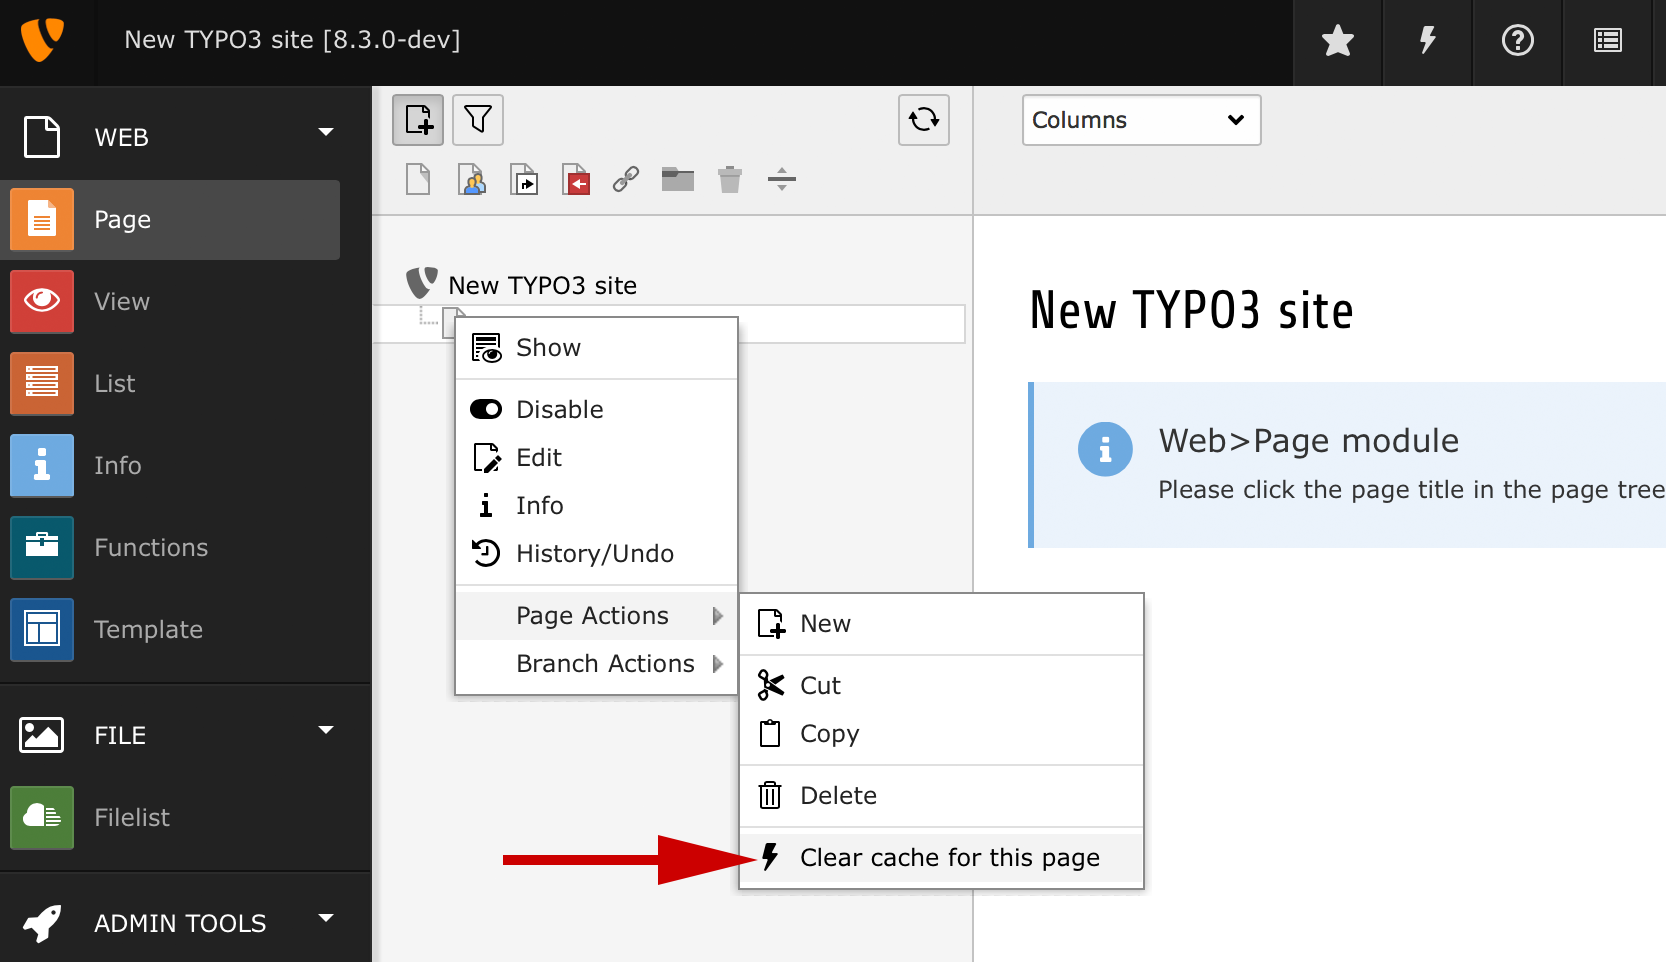
\includegraphics[width=0.70\linewidth]{BackendUserInterface/20446.png}
	\end{figure}

\end{frame}

% ------------------------------------------------------------------------------
% LTXE-SLIDE-START
% LTXE-SLIDE-UID:		72dde6ef-007a2756-22324bc6-fd8072c9
% LTXE-SLIDE-ORIGIN:	e24e593c-fe9bcff9-c386db3a-79491de1 English
% LTXE-SLIDE-TITLE:		Workspaces (1)
% ------------------------------------------------------------------------------
\begin{frame}[fragile]
	\frametitle{Gebruikersinterface backend}
	\framesubtitle{Herbouwde werkruimtes (1)}

	\begin{itemize}

		\item De module werkruimtes om klaarstaande inhoud te beheren is herschreven
			en past nu beter binnen het uiterlijk van de backend.

		\item Redacteuren merken direct dat het beter past doordat het uiterlijk nu
		 	gebaseerd is op Twitter Bootstrap en jQuery

		\item Hierdoor is er ook een verbetering qua performance en een grote stap
		 	voorwaards naar een schonere en snellere TYPO3 backend met minder JavaScript

	\end{itemize}

\end{frame}

% ------------------------------------------------------------------------------
% LTXE-SLIDE-START
% LTXE-SLIDE-UID:		1c14bb36-26cfb8c2-55b9674c-76b00298
% LTXE-SLIDE-ORIGIN:	fe9bcff9-e24e593c-79491de1-c386db3a English
% LTXE-SLIDE-TITLE:		Workspaces (2)
% ------------------------------------------------------------------------------
\begin{frame}[fragile]
	\frametitle{Gebruikersinterface backend}
	\framesubtitle{Herbouwde werkruimtes (2)}

	Screenshots van de module werkruimtes:

	\begin{figure}
		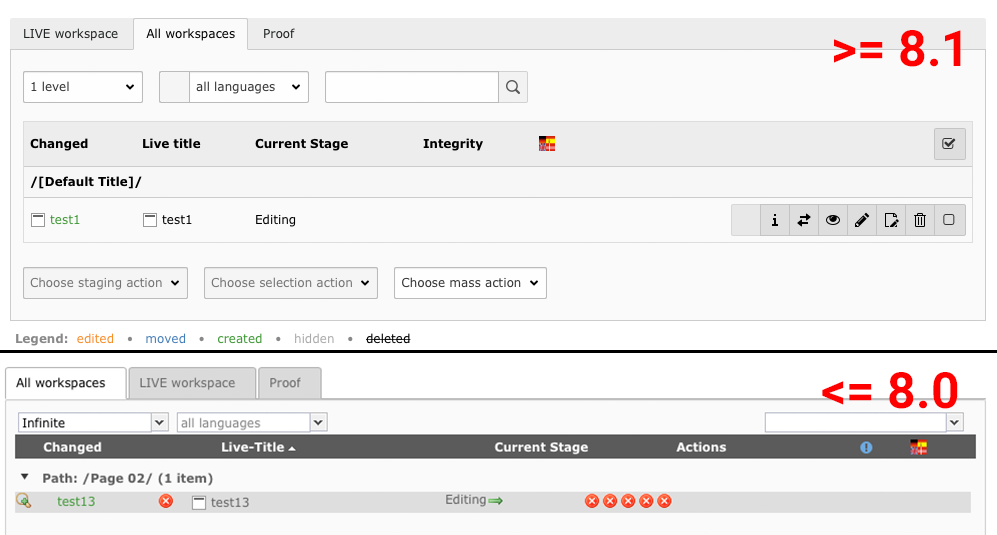
\includegraphics[width=0.85\linewidth]{BackendUserInterface/workspaces.png}
	\end{figure}

\end{frame}

% ------------------------------------------------------------------------------
% LTXE-SLIDE-START
% LTXE-SLIDE-UID:		6a72c49c-28841046-14c871c7-282b2dd4
% LTXE-SLIDE-ORIGIN:	c9dc360d-cf218f95-03f53731-03d821ad English
% LTXE-SLIDE-TITLE:		#78383: Field positions in tabs streamlined (TCA)
% ------------------------------------------------------------------------------
\begin{frame}[fragile]
	\frametitle{Gebruikersinterface backend}
	\framesubtitle{Positie en volgorde van elementen}

	\begin{itemize}
		\item De volgorde en positie van bepaalde velden in de backend is geoptimaliseerd
		\item Het doel is aan te sluiten bij de verwachting van gebruikers waar veelgebruikte opties te vinden zijn
		\item Dit is vooral belangrijk voor veelgebruikte velden en algemene categorieën die door vele records gedeeld worden
		\item Auteurs van extensie wordt aangeraden om de specifieke posities en volgorde van elementen in
		 	de \href{https://docs.typo3.org}{official documentation} te volgen.

			% TODO: update link above (waiting for Doc and Core Team to finish documentation)

	\end{itemize}

	\begin{itemize}
		\item \textit{Een consistente backend is belangrijk!} :-)
	\end{itemize}

\end{frame}

% ------------------------------------------------------------------------------
